A partir das simulações para o ano de 2022, foi construído um dashboard para analisar os KPIs (\textit{key performance indicators}) e ajudar na tomada de decisão do gerente da empresa. Os indicadores analisados para a tomada de decisão foram: porcentagem de atendimentos realizados em até um minuto, número de chamados no dia, tempo de espera, tempo de atendimento, taxa de desistência, definida como o percentual de ligações que duraram menos de 30 segundos, e o percentual de utilização dos atendentes. A Figura \ref*{fig: dashboard} mostra a parte do dashboard que permite analisar a meta estabelecida pela gerência e o número de chamados atendidos no dia selecionado, neste caso, 31 de dezembro de 2021.

\begin{figure}[H]
    \centering
    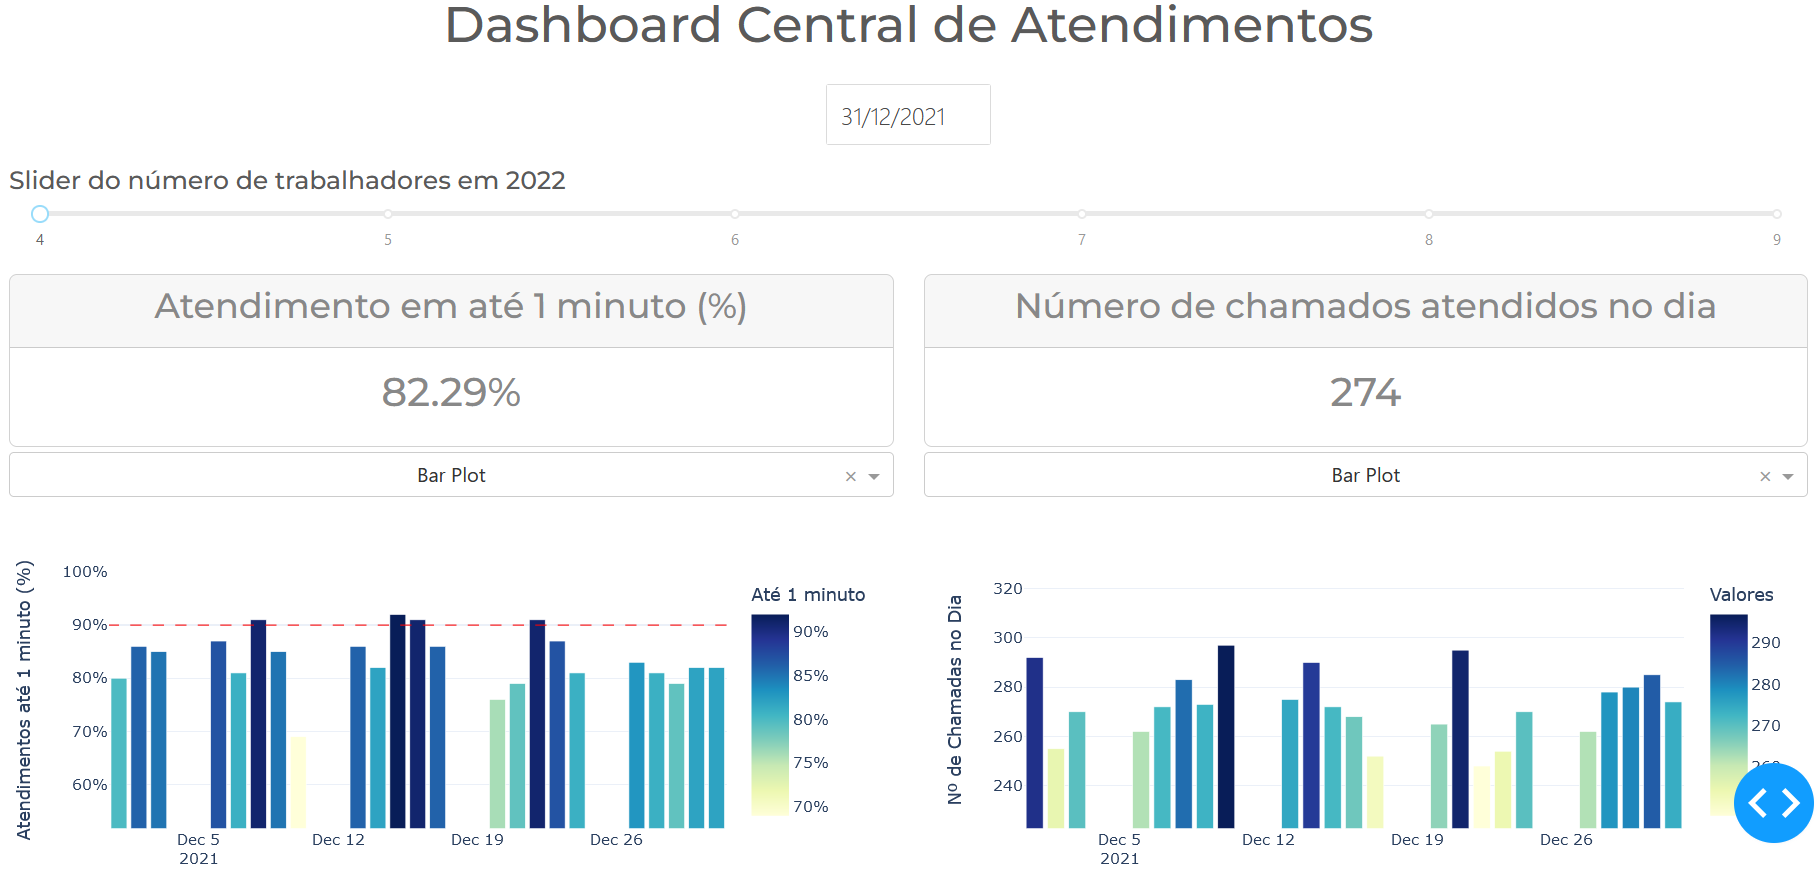
\includegraphics[scale=0.45]{propostas/dashboard.png}
    \caption{Estrutura do dashboard desenvolvido para a gerência da empresa}
    \label{fig: dashboard}
\end{figure}

\subsection{Contratação de atendentes}
Neste dashboard, os dados para o ano de 2021 são os fornecidos pela empresa, e, portanto, não são passíveis de alterações. A partir de 2022 é possível alterar o número de trabalhadores para avaliar o comportamento do sistema. Considerando que não haja tolerância ao descumprimento da meta, isto é, visando manter todos os dias do mês com um percentual de atendimento em até um minuto acima de 90\%, foi desenvolvida a Tabela \ref*{tab: funcionarios-2022} com o número de atendentes necessários para cumprimento da meta de ligações a cada mês de 2022. Como o sistema que trabalhou o ano de 2021 com apenas 4 atendentes já estava sobrecarregado, é necessária a contratação de pelo menos 2 atendentes em janeiro, para corrigir o descumprimento da meta dos meses anteriores. Após isso, deve ser contratado outro atendente em fevereiro, trabalhando com 7 atendentes até o mês de setembro. As últimas contratações do ano ocorrem em outubro e dezembro.

\begin{table}[H]
    \centering
    \begin{tabular}{|l|r|r|}
    \hline
    \textbf{Mês} & \multicolumn{1}{l|}{\textbf{Trabalhadores}} & \multicolumn{1}{l|}{\textbf{Contratações}} \\ \hline
    Janeiro & 6 & 2 \\ \hline
    Fevereiro & 7 & 1 \\ \hline
    Março & 7 & 0 \\ \hline
    Abril & 7 & 0 \\ \hline
    Maio & 7 & 0 \\ \hline
    Junho & 7 & 0 \\ \hline
    Julho  & 7 & 0 \\ \hline
    Agosto & 7 & 0 \\ \hline
    Setembro & 7 & 0 \\ \hline
    Outubro & 8 & 1 \\ \hline
    Novembro & 8 & 0 \\ \hline
    Dezembro & 9 & 1 \\ \hline
    \end{tabular}
    \caption{Funcionários necessários e contratações para cada mês de 2022 antecipando o crescimento na demanda para cumprimento da meta}
    \label{tab: funcionarios-2022}
    \end{table}
    
Outra possibilidade para o gerente da central de atendimentos é, ao invés de se antecipar à demanda para a contratação de atendentes, trabalhando assim com capacidade ociosa, contratar novos atendentes apenas quando necessário, isto é, tolerando no máximo uma ocasião no mês em que a meta de desempenho de 90\% das chamadas atendidas em até um minuto não é cumprida. A Tabela \ref*{tab: funcionarios-2022-economico} representa este cenário.\\
No caso, apesar do mês de fevereiro apresentar um dia em que a meta não é cumprida com 6 atendentes, os meses de março e abril não apresentam este problema, e a contratação do sétimo atendente poderia ser postergada para junho, proporcionando economias para a empresa. Essa postura conservadora de contratações considera que a simulação não representa completamente a realidade, e, portanto, pode ser interessante avaliar o comportamento do sistema real ao longo do tempo antes de decidir pela necessidade da contratação. 

\begin{table}[H]
    \centering
    \begin{tabular}{|l|r|r|}
    \hline
    \textbf{Mês} & \multicolumn{1}{l|}{\textbf{Trabalhadores}} & \multicolumn{1}{l|}{\textbf{Contratações}} \\ \hline
    Janeiro & 6 & 2 \\ \hline
    Fevereiro & 6 & 0 \\ \hline
    Março & 6 & 0 \\ \hline
    Abril & 6 & 0 \\ \hline
    Maio & 6 & 0 \\ \hline
    Junho & 7 & 1 \\ \hline
    Julho  & 7 & 0 \\ \hline
    Agosto & 7 & 0 \\ \hline
    Setembro & 7 & 0 \\ \hline
    Outubro & 8 & 1 \\ \hline
    Novembro & 8 & 0 \\ \hline
    Dezembro & 8 & 0 \\ \hline
    \end{tabular}
    \caption{Funcionários necessários e contratações para cada mês de 2022 utilizando abordagem conservadora}
    \label{tab: funcionarios-2022-economico}
    \end{table}

As alternativas de contratação propostas devem ser consideradas pela gerência e adequadas às necessidades da empresa, a depender do nível de tolerância ao não cumprimento da meta dentro de um mês e da disponibilidade e custo de contratação dos trabalhadores nos meses determinados. Pode ser mais interessante, por exemplo, a contratação de 3 atendentes em janeiro de 2022, ao invés de 2 em janeiro e mais um em fevereiro, devido a possíveis economias com recrutamento e treinamento de funcionários.

\subsection{Subcontratação}
A depender do tipo de problema tratado nessa central de atendimentos, pode ser possível a subcontratação de outra central, permitindo a terceirização do atendimento de parte das ligações recebidas. Essa estratégia pode ser economicamente interessante em relação à contratação direta de novos atendentes, mas pode ser inaqueada para as especificidades da empresa.

\subsection{Redução dos tempos de atendimento}
Há a possibilidade de aumentar diretamente a eficiência dos atendentes disponíveis, reduzindo o tempo médio de atendimento. Isto pode ser atingido por meio de treinamentos que permitam solucionar os problemas dos clientes mais rapidamente. Pode ser necessário para a empresa um mapeamento de processos que possibilite destacar as melhores práticas de atendimento, assim como avaliar as condições atuais de trabalho para propor mudanças que aumentem a eficiência dos trabalhadores.

\subsection{Utilização de chatbots}
É possível reduzir a parcela das ligações classificadas como desistência, aquelas com duração inferior a 30 segundos, ao implementar um sistema de triagem de ligações que utiliza tecnologias como chatbots para lidar com chamadas mais simples e liberar recursos para chamadas mais complexas. Isso permite que os clientes acessem uma alternativa de atendimento mais rapidamente e esperem por um atendente apenas quando necessário.

\subsection{Classificação efetiva dos tipos de ligação recebidos}
Ficou evidente na análise do histórico de atendimentos que a atual classificação dos tipos de ligação não ajudou na resolução dos problemas da empresa. Um estudo posterior pode ser empregado no sentido de aprimorar a classificação e análise dos tipos de chamadas recebidas de acordo com a complexidade, auxiliando no processo de triagem das ligações que podem ser atendidas por chatbots.

\subsection{Melhoria da comunicação com os clientes}
A melhoria da comunicação com os clientes, no sentido de mantê-los informados sobre o status da chamada, pode reduzir a quantidade de desistências e a frustração. Neste período de espera para o atendimento, também é possível orientar o cliente a se preparar para fornecer informações relevantes à resolução do seu problema, assim, mesmo que o chatbot não seja capaz de resolvê-lo, o tempo de atendimento pode ser reduzido.